\documentclass{amsart}
\usepackage{array}
\usepackage{multicol}
\usepackage{longtable}
\usepackage{subfig,enumerate}
\usepackage{ragged2e, color}
\usepackage{amsmath,amssymb,amsthm,graphicx, graphics}
\usepackage[all]{xy}
\usepackage[pdfpagelabels]{hyperref}                 % For creating hyperlinks in cross references

\usepackage{pgf,tikz}
\usepackage{mathrsfs,multicol}
\usetikzlibrary{arrows}

%CALCULUS
\newcommand{\dydx}{\frac{dy}{dx}}
\newcommand{\ddx}{\frac{d}{dx}}
\newcommand{\ddt}{\frac{d}{dt}}
\newcommand{\dd}[2]{\frac{d#1}{d#2}}
\newcommand{\uv}{\vec{u}}
\newcommand{\vv}{\vec{v}}
\newcommand{\wv}{\vec{w}}
\newcommand{\av}{\vec{a}}
\newcommand{\bv}{\vec{b}}
\newcommand{\rvt}{\vec{r}(t)}
\newcommand{\rvtp}{\vec{r}\,'(t)}
\newcommand{\vvp}{\vec{v}\,'(t)}
\newcommand{\uvp}{\vec{u}\,'(t)}
\newcommand{\fv}[1]{\langle #1 \rangle} 
\newcommand{\ihat}{\mathbf{\hat{\textbf{\i}}}}
\newcommand{\jhat}{\mathbf{\hat{\textbf{\j}}}}
\newcommand{\khat}{\mathbf{\hat{\textbf{k}}}}
\newcommand{\la}{\left\langle\,}
\newcommand{\ra}{\,\right\rangle}
\newcommand{\dotp}{\hspace{.25em}\begin{picture}(-1,1)(-1,-3)\circle*{2}\end{picture}\hspace{.5em} }
\newcommand{\proj}[2]{\textrm{proj}_{\,#2}\:#1 }
\newcommand{\compp}[2]{\textrm{comp}_{\,#2}\:#1 }
\newcommand{\pder}[2]{\frac{\partial #1}{\partial #2}}
\newcommand{\ppder}[3]{\frac{\partial^2 #1}{\partial #3\,\partial #2}}
\newcommand{\V}[1]{\vec{#1}}
\newcommand{\ds}{\displaystyle}
\newcommand{\curl}{\mathrm{curl}\,}
\renewcommand{\div}{\mathrm{div}\,}

%STANDARD SETS
\newcommand{\R}{\mathbb{R}}
\newcommand{\Q}{\mathbb{Q}}
\newcommand{\Z}{\mathbb{Z}}
\newcommand{\C}{\mathbb{C}}
\newcommand{\N}{\mathbb{N}}
\newcommand{\F}{\mathbb{F}} %finite field

%GENERAL
\newcommand{\inv}{^{-1}}
\newcommand{\del}{\partial}
\newcommand{\by}{\times}

\newcommand{\comp}{\circ}

\newcommand{\infunion}{\bigcup_{i=1}^\infty}
\newcommand{\infcap}{\bigcap_{i=1}^\infty}
\newcommand{\floor}[1]{\lfloor #1 \rfloor}

\newcommand{\blankline}{\vspace{.1in}}
\newcommand{\fillin}[1]{\underline{\hspace{#1 in}}}


\parindent 1cm
\parskip 0.2cm
\topmargin -1.5cm

\oddsidemargin -1cm
\evensidemargin -1cm
\textwidth 18.5cm
\textheight 23.5cm
\newtheorem{theorem}{Theorem}
\newtheorem{proposition}[theorem]{Proposition}
\newtheorem{corollary}[theorem]{Corollary}
\newtheorem{lemma}[theorem]{Lemma}
\newtheorem{remark}[theorem]{Remark}



\theoremstyle{definition}
\newtheorem{formula}[theorem]{Formula}
\newtheorem{example}{Example}
\newtheorem{definition}{Definition}

\makeindex



\title{Handout to accompany 3D-printed models}

\author{Dr.~Eric Bancroft, Grove City College  }

\date{ Summer 2026 }



%\newlength\boxedblankwidth
%\setlength{\boxedblankwidth}{\textwidth}
%\advance\boxedblankwidth by -\leftmargin
%\newcommand\boxedblank[2][1in]{\fbox{\raisebox{0pt}[\height][#1]{\parbox[t]{\boxedblankwidth}{#2}}}}
%
%\newlength\textwidthinlist
%\newcommand\computetextwidthinlist{\textwidthinlist=\textwidth
%                                   \advance\textwidthinlist by -\leftmargin
%                                   \advance\textwidthinlist by -\rightmargin}



%%%%%%%%%%%%
% -- DOCUMENT -- %
%%%%%%%%%%%%

\begin{document}
%\maketitle
\section*{Region 3}
Set up all six orders of integration for \[\iiint\limits_{R_3} f(x,y,z) \, dV,\] where $R_3$ is the region bounded by 
\[y=x,\ y=\sqrt{2-x^2},\ z = 2x^2 + y^2,\ z=4-y^2,\ \text{and }  0 \leq x \leq 1.\]

\begin{figure}[!ht]
\vspace{-1em}
	\centering
	\begin{tabular}{{m{5cm}m{9.25cm}}}
		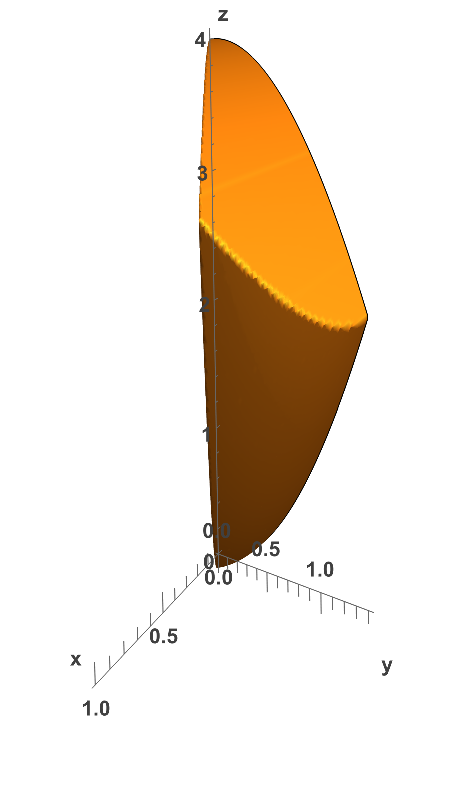
\includegraphics[width=.25\textwidth]{Solid3Full} &
		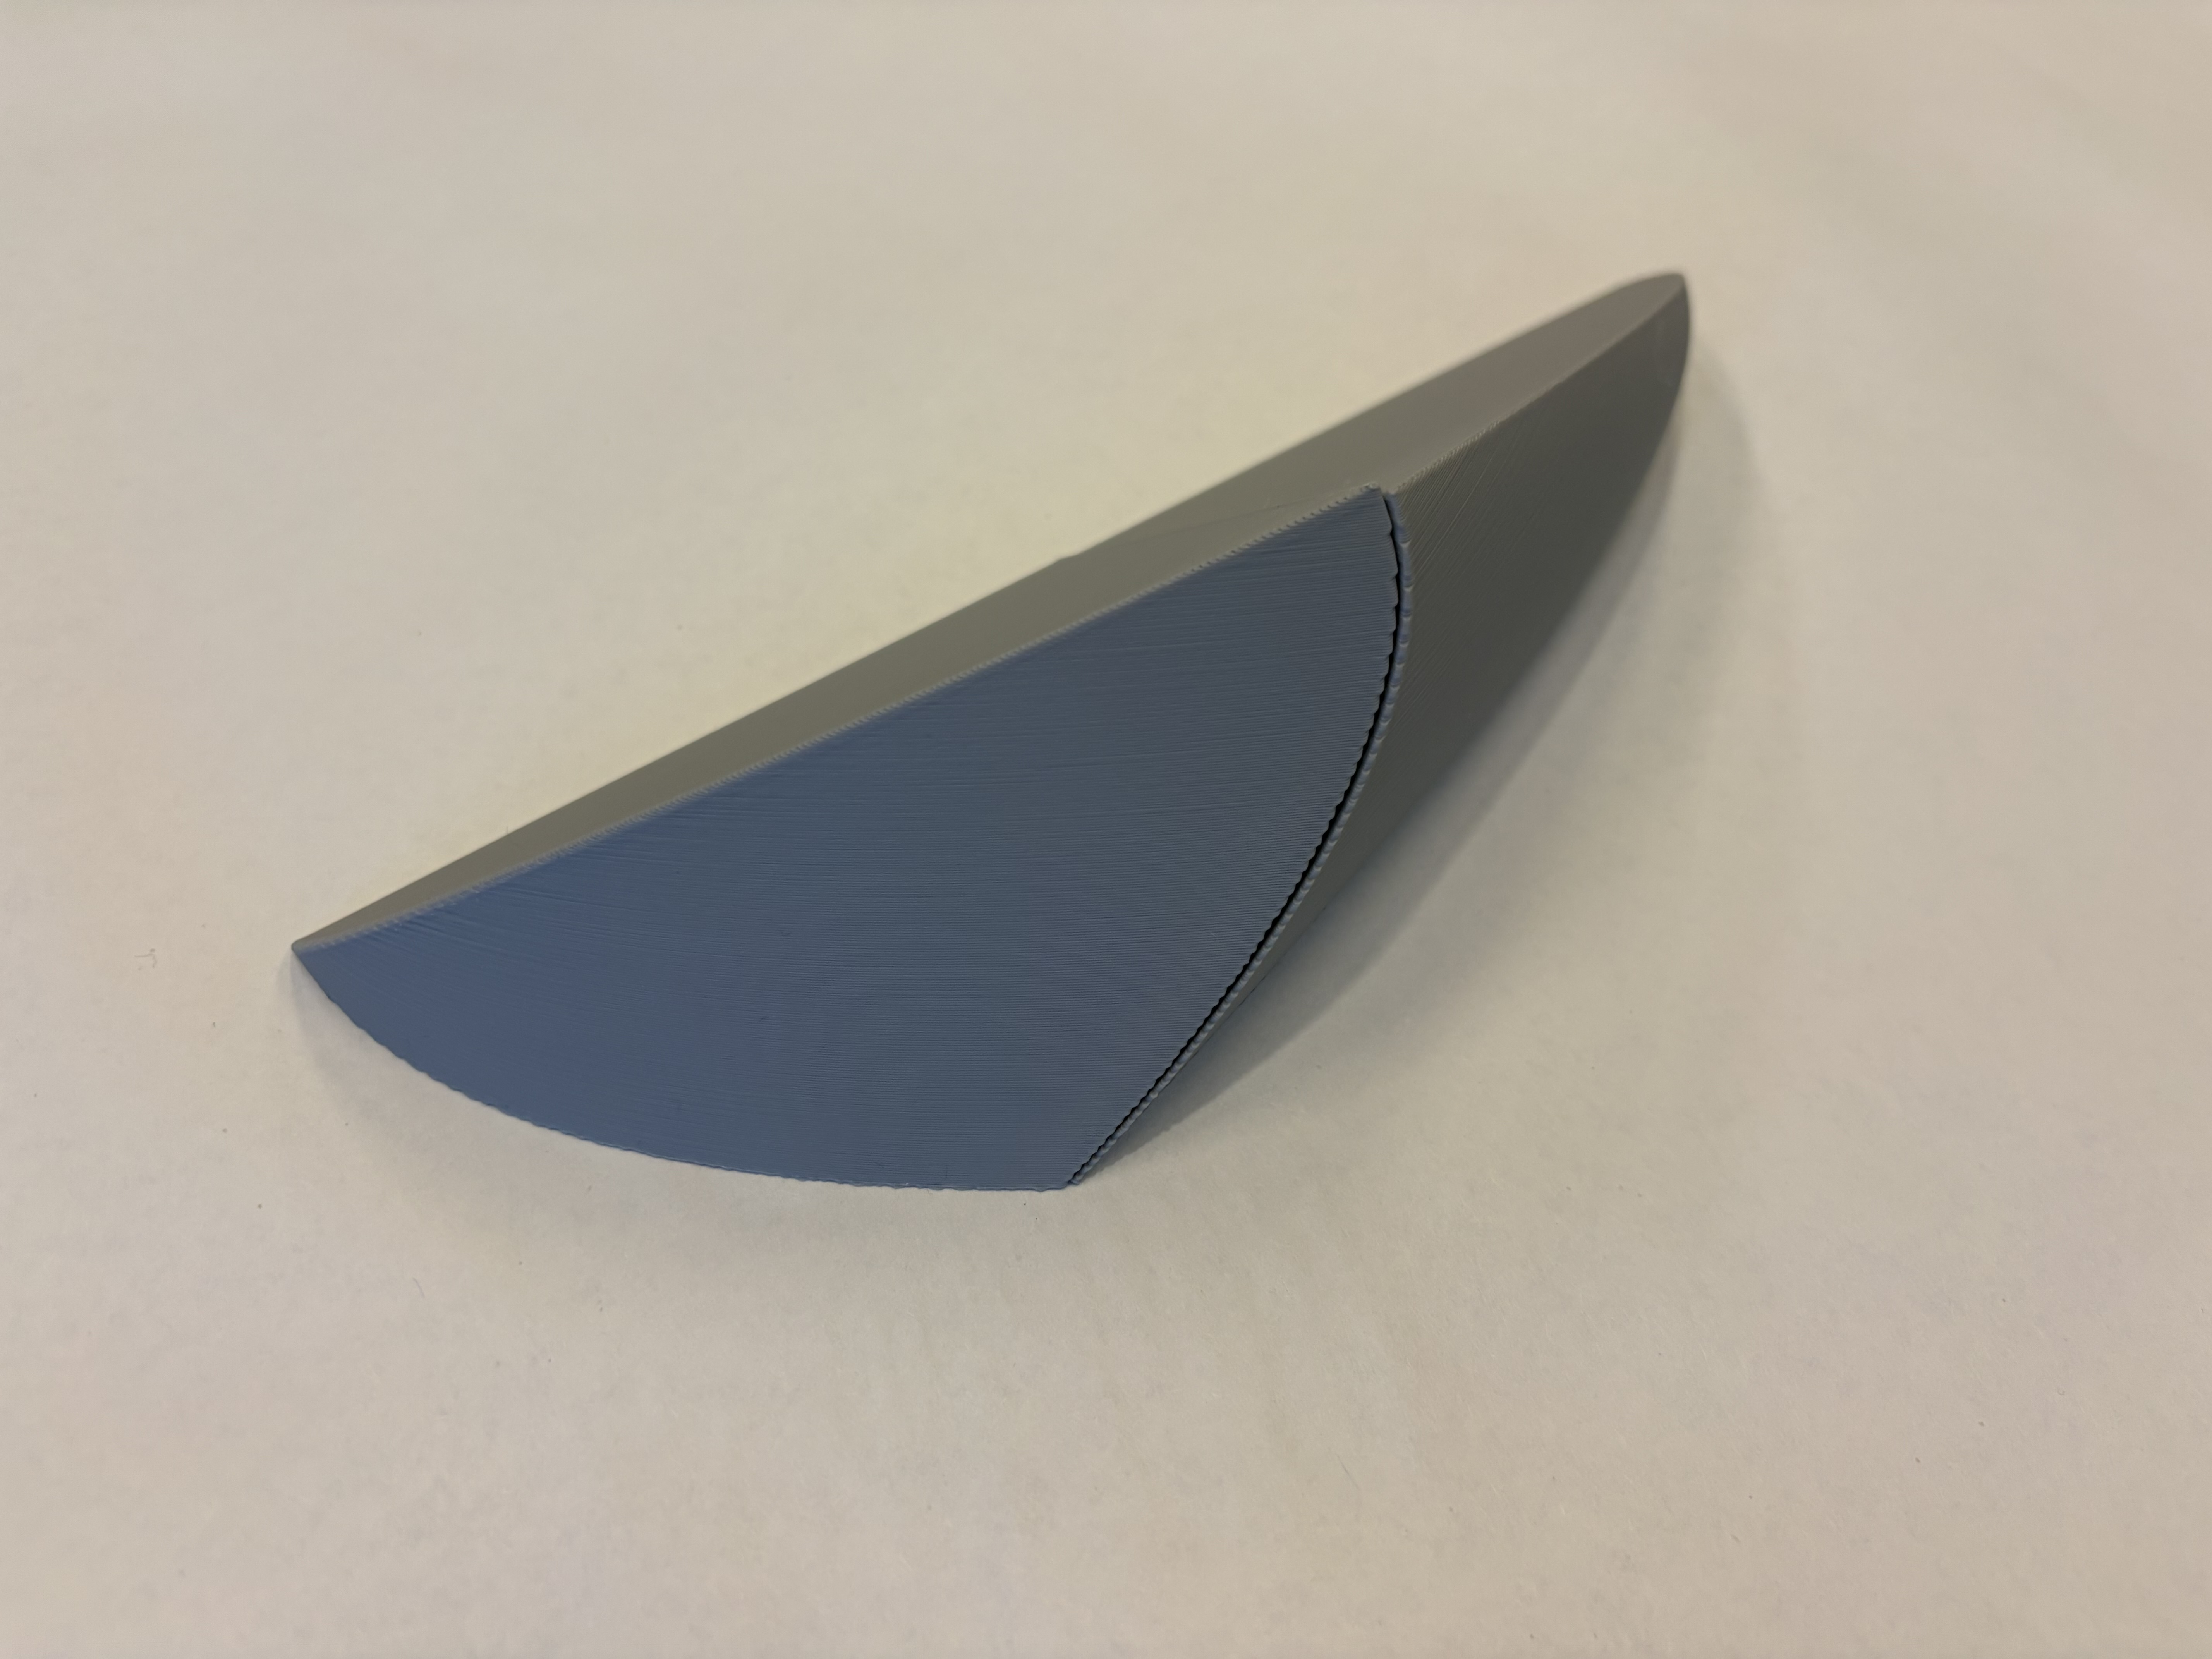
\includegraphics[width=.5\textwidth]{Solid3Print}
	\end{tabular}
	\caption{Computer-modeled and 3D-printed views of $R_3$}
\end{figure}

\begin{figure}[!ht]
\vspace{-1em}
	\centering
	\begin{tabular}{ccc}
		\subfloat[$xy$-projection]{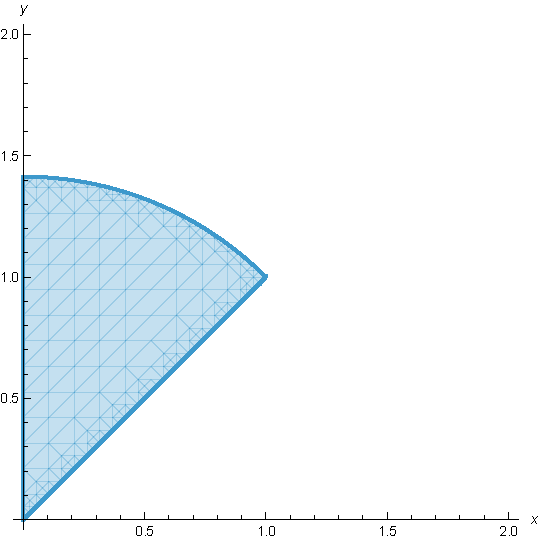
\includegraphics[width=.15\textwidth]{Solid3XYProj}} &
		\subfloat[$xz$-projection]{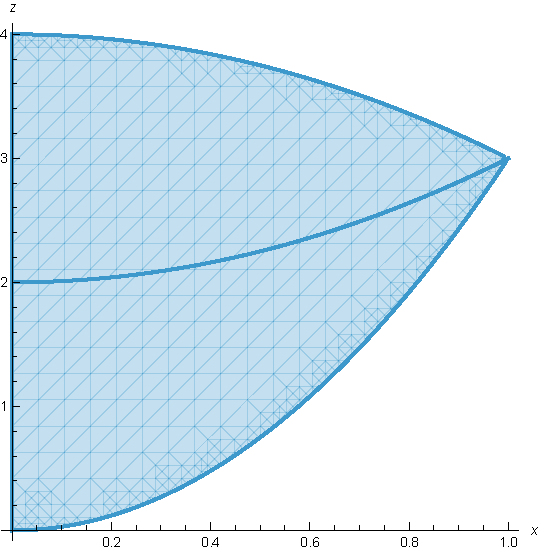
\includegraphics[width=.15\textwidth]{Solid3XZProj}} &
		\subfloat[$yz$-projection]{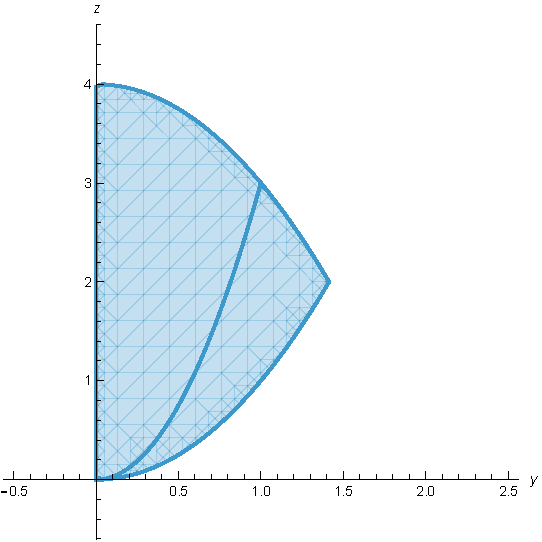
\includegraphics[width=.15\textwidth]{Solid3YZProj}}
	\end{tabular}
	\caption{Projections of $R_3$ into the three coordinate planes.}%\label{projE2}
\end{figure}

\clearpage

\vspace{1em}

The following triple integrals represents integrating over the region using the $xy$-projection:

\[\int_{1}^{\sqrt{2}}\int_{0}^{\sqrt{2-y^2}}\int_{2x^2+y^2}^{4-y^2} f(x,y,z)\, dz\, dx\, dy \ + \
\int_{0}^{1}\int_{0}^{y}\int_{2x^2+y^2}^{4-y^2} f(x,y,z)\, dz\, dx\, dy\]
or 
\[\int_{0}^{1}\int_{x}^{\sqrt{2-x^2}}\int_{2x^2+y^2}^{4-y^2} f(x,y,z)\, dz\, dy\, dx\]

\vspace{0.5cm}
The following triple integrals represent integrating over the region using the $xz$-projection:
\begin{align*}
&\int_{3}^{4}\int_{0}^{\sqrt{4-z}}\int_{x}^{\sqrt{4-z}} f(x,y,z)\, dy\, dx\, dz  + 
\int_{2}^{3}\int_{0}^{\sqrt{z-2}}\int_{x}^{\sqrt{4-z}} f(x,y,z)\, dy\, dx\, dz\\
&+ \int_{2}^{3}\int_{\sqrt{z-2}}^{\sqrt{\frac{z}{3}}}\int_{x}^{\sqrt{z-2x^2}} f(x,y,z)\, dy\, dx\, dz
+\int_{0}^{2}\int_{0}^{\sqrt{\frac{z}{3}}}\int_{x}^{\sqrt{z-2x^2}} f(x,y,z)\, dy\, dx\, dz
\end{align*}
\vspace{1em}
or
\[\int_{0}^{1}\int_{x^2+2}^{4-x^2}\int_{x}^{\sqrt{4-z}} f(x,y,z)\, dy\, dz\, dx  + 
\int_{0}^{1}\int_{3x^2}^{x^2+2}\int_{x}^{\sqrt{z-2x^2}} f(x,y,z)\, dy\, dz\, dx\]

\vspace{0.5cm}
The following triple integrals represent integrating over the region using the $yz$-projection:

\begin{align*}
& \int_{3}^{4}\int_{0}^{\sqrt{4-z}}\int_{0}^{y} f(x,y,z)\, dx\, dy\, dz
+ \int_{0}^{3}\int_{0}^{\sqrt{\frac{z}{3}}}\int_{0}^{y} f(x,y,z)\, dx\, dy\, dz  \\
&+ \int_{2}^{3}\int_{\sqrt{\frac{z}{3}}}^{\sqrt{4-z}}\int_{0}^{\sqrt{\frac{1}{2}(z-y^2)}} f(x,y,z)\, dx\, dy\, dz
+ \int_{0}^{2}\int_{\sqrt{\frac{z}{3}}}^{\sqrt{z}}\int_{0}^{\sqrt{\frac{1}{2}(z-y^2)}} f(x,y,z)\, dx\, dy\, dz
\end{align*}
or 
%\begin{align*}
%& \int_{0}^{1}\int_{3y^2}^{4-y^2}\int_{0}^{y} f(x,y,z)\, dx\, dz\, dy +
%\int_{0}^{1}\int_{y^2}^{3y^2}\int_{0}^{\sqrt{\frac{1}{2}(z-y^2)}} f(x,y,z)\, dx\, dz\, dy \\
%&+ \int_{1}^{\sqrt{2}}\int_{y^2}^{4-y^2}\int_{0}^{\sqrt{\frac{1}{2}(z-y^2)}} f(x,y,z)\, dx\, dz\, dy
%\end{align*}
\[\int_{0}^{1}\int_{3y^2}^{4-y^2}\int_{0}^{y} f(x,y,z)\, dx\, dz\, dy +
\int_{0}^{1}\int_{y^2}^{3y^2}\int_{0}^{\sqrt{\frac{1}{2}(z-y^2)}} f(x,y,z)\, dx\, dz\, dy + \int_{1}^{\sqrt{2}}\int_{y^2}^{4-y^2}\int_{0}^{\sqrt{\frac{1}{2}(z-y^2)}} f(x,y,z)\, dx\, dz\, dy\]

%\item $\ds\int\qquad \int\qquad\int\quad f(x,y,z) \,dx\, dy\, dz$
%\item $\ds\int\qquad \int\qquad\int\quad f(x,y,z) \,dx\, dz\, dy$
%\item $\ds\int\qquad \int\qquad\int\quad f(x,y,z) \,dy\, dx\, dz$
%\item $\ds\int\qquad \int\qquad\int\quad f(x,y,z) \,dy\, dz\, dx$
%\item $\ds\int\qquad \int\qquad\int\quad f(x,y,z) \,dz\, dx\, dy$
%\item $\ds\int\qquad \int\qquad\int\quad f(x,y,z) \,dz\, dy\, dx$

\vspace{1em}
All of these triple integrals evaluate to $\frac{\pi}{2}$ when $f(x,y,z) = 1$.
\end{document}